%\pdfobjcompresslevel=0
%\pdfminorversion=4
\documentclass[aspectratio=43]{beamer}

\usepackage{hyperref}
\usepackage{multimedia}
\usepackage[textsize=tiny]{todonotes}
\presetkeys%
{todonotes}%
{inline}{}


%\usepackage[pdftex]{graphicx}
%\usepackage{graphviz}
\usepackage{graphviz}
%===Pick Theme===
\usetheme{Warsaw}
\usecolortheme{beaver}
\useoutertheme{infolines}
\useinnertheme{circles}

%===Customize Theme=== %
\setbeamercolor{item}{fg=darkred}
\setbeamertemplate{itemize subitem}{$\circ$}
\setbeamercolor*{block title}{fg=white, bg=darkred}
\setbeamercolor*{block body}{bg=lightgray}

%===Set the covered style=== %
\setbeamercovered{transparent}
%===Set the bib reference key style=== %
\setbeamertemplate{bibliography item}[text]
%===Disable navigation bar=== %
\setbeamertemplate{navigation symbols}{}%remove navigation symbols

\usepackage{minted}
\setminted[python]{bgcolor=bg,fontsize=\scriptsize,linenos,xleftmargin=8pt}
\setminted[xml]{bgcolor=bg,fontsize=\scriptsize,linenos,xleftmargin=8pt}

\setmintedinline[python]{bgcolor=bg,fontsize=\scriptsize}
\setmintedinline[bash]{bgcolor=bg,fontsize=\scriptsize}
\setmintedinline[text]{bgcolor=bg,fontsize=\scriptsize}
\setmintedinline[xml]{bgcolor=bg,fontsize=\scriptsize}

\newcommand{\pyinline}[1]{\mintinline{python}{#1}}
\newcommand{\bashinline}[1]{\mintinline{bash}{#1}}
\newcommand{\inline}[1]{\mintinline{text}{#1}}
%===Logos=== %

%\usepackage{pgf}
%\logo{\pgfputat{\pgfxy(-1,7)}{\pgfbox[center,base]{
\includegraphics[height=0.5in]{fig/duckietown_logo}}}}

\logo{
\includegraphics[height=0.5in]{fig/duckietown_logo}}
\titlegraphic{ %
\centering

\includegraphics[height=1.8in]{fig/duckietown_logo}%\hspace{2ex}
%\raisebox{-0.75in}{
\includegraphics[height=1.5in]{fig/indigoigloo_600.png}}
} %

% \author[Michael ``Misha'' Novitzky]{Michael ``Misha'' Novitzky}
\author[S.-Y.Liu, M. Novitzky]{Shih-Yuan Liu, Michael ``Misha'' Novitzky}
\title[ROS in Duckietown]{Robot Operating System (ROS) in Duckietown}
\institute[Duckietown MIT]{Duckietown, MIT}
\date[Feb. 16th, 2016]{February 16th 2016}

\begin{document}
\definecolor{bg}{rgb}{0.95,0.95,0.95}

\begin{frame}[plain,label=titlepage,noframenumbering] %[plain,noframenumbering] will not show the header and footer
	\titlepage
\end{frame}

\begin{frame}[label=overview]{Overview}
	\tableofcontents
	%\tableofcontents[sectionstyle=show/shaded,subsectionstyle=show/shaded/shaded]
\end{frame}

\section{Introduction to Middlewares in Duckietown}

\begin{frame}{Duckiebot Videos}
\begin{columns}
	\begin{column}{0.55\textwidth}
		Shih-Yuan - how do I embed \alert{videos} in latex? Probably not right? Output is PDF. \todo{See videos slide}
		\begin{itemize}
			\item Output line filter?
			\item Open-loop intersection?
			\item Lane following awesomeness -- for sure
		\end{itemize}
	\end{column}
	\begin{column}{0.45\textwidth}
		\centering
		
\includegraphics[width=\textwidth]{fig/indigoigloo_600.png}
	\end{column}
\end{columns}
\end{frame}

\begin{frame}{Videos}
\begin{center}
  \movie[showcontrols=true]{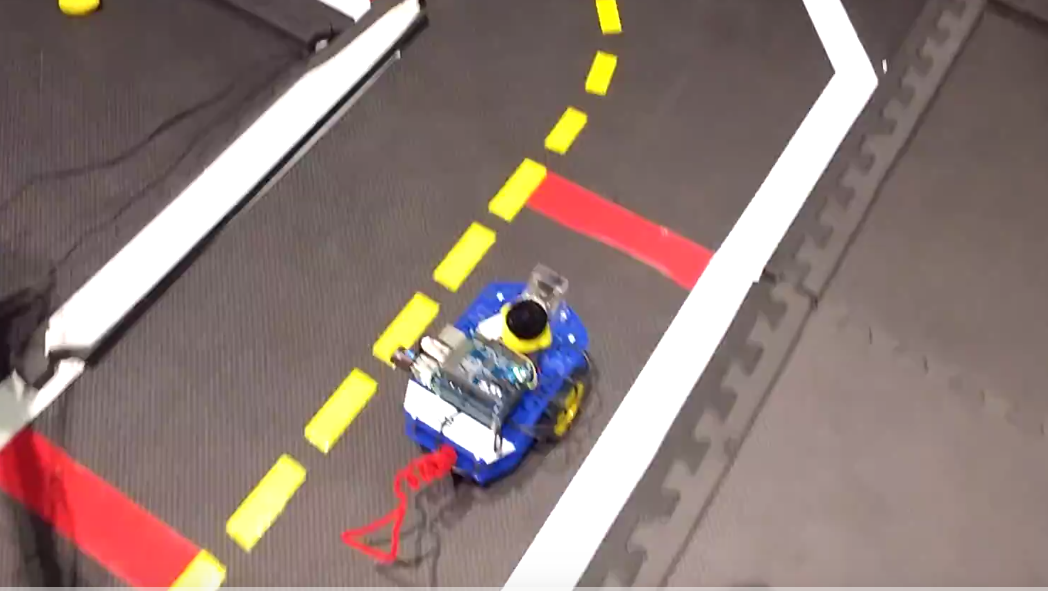
\includegraphics[width=0.8\textwidth]{videos/lane_following_1.png}}{videos/lane_following_1.mp4}
\end{center}
\end{frame}

\begin{frame}{Videos}
\begin{center}
  \movie[showcontrols=true]{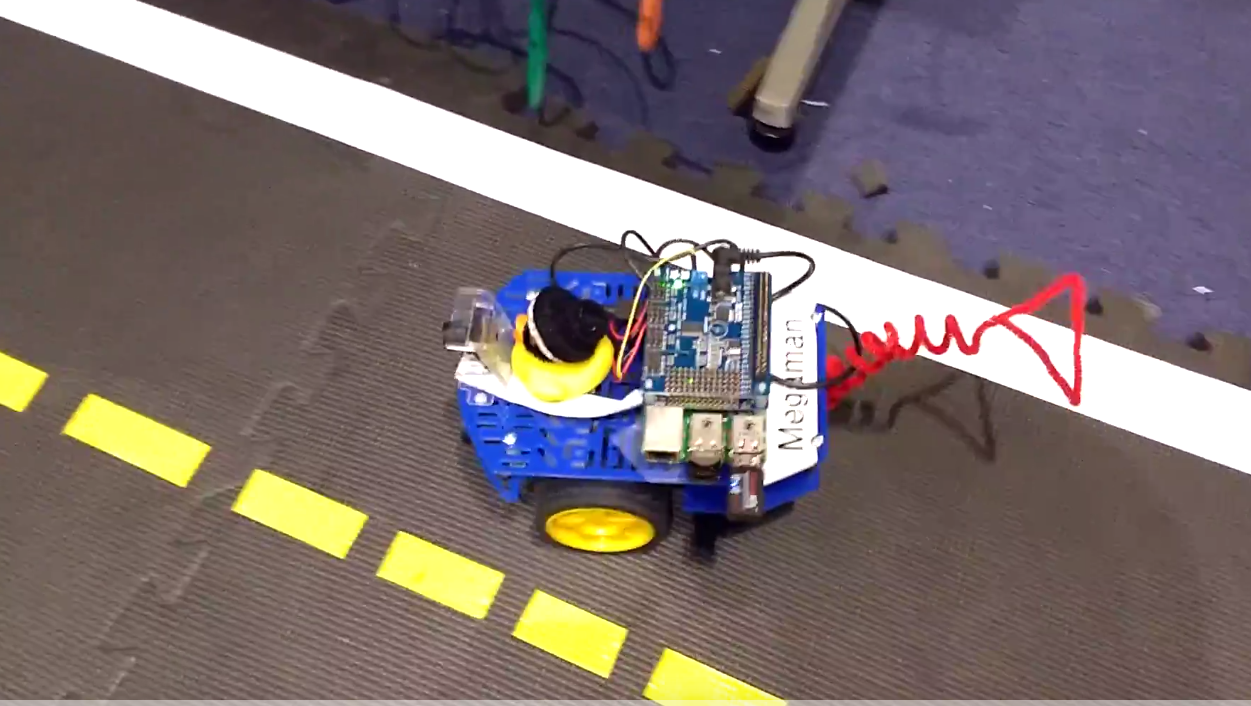
\includegraphics[width=0.8\textwidth]{videos/lane_following_2.png}}{videos/lane_following_2.mp4}
\end{center}
\end{frame}

\begin{frame}{Team Success}
\begin{columns}
	\begin{column}{0.55\textwidth}
		\begin{itemize}
			\item No man is an island
			\item \alert{Shih-yuan} (glue)
\item Team members: Liam, Andrea, Hang, Misha, etc
		\end{itemize}
	\end{column}
	\begin{column}{0.45\textwidth}
		\centering
		
\includegraphics[width=\textwidth]{fig/indigoigloo_600.png}
	\end{column}
\end{columns}

\end{frame}


\begin{frame}{Why Shih-Yaun = glue?}
\begin{columns}
	\begin{column}{0.55\textwidth}
Historical note:
		\begin{itemize}
			\item Want to advance state of the art
                        \item How parts talk to each other?
                        \item Build infrastructure
			\item Throw away 
		\end{itemize} \end{column} \begin{column}{0.45\textwidth} \centering 
\includegraphics[width=\textwidth]{fig/indigoigloo_600.png} \end{column}
\end{columns}

\end{frame}


\begin{frame}{What problems did they encounter?}
\begin{columns}
	\begin{column}{0.55\textwidth}
Thought process:
		\begin{itemize}
			\item One giant loop?
                        \item Many small pieces?
                        \item Reusable? 
		\end{itemize} \end{column} \begin{column}{0.45\textwidth} \centering 
\includegraphics[width=\textwidth]{fig/indigoigloo_600.png} \end{column}
\end{columns}

\end{frame}

\section{Middleware}
\begin{frame}{Enter the Middleware}
\begin{columns}
	\begin{column}{0.55\textwidth}
An abstraction:
		\begin{itemize}
			\item Not the operating system
                        \item Not the application
                        \item Right in the middle
		\end{itemize} \end{column} \begin{column}{0.45\textwidth} \centering 
\includegraphics[width=\textwidth]{fig/indigoigloo_600.png} \end{column}
\end{columns}

\end{frame}



\begin{frame}{What do we gain?}
\begin{columns}
	\begin{column}{0.55\textwidth}
We benefit:		\begin{itemize}
			\item Abstraction from hardware
                        \item Portable
                        \item Reusable
                        \item Saves time
                        \item Saves money
		\end{itemize} \end{column} \begin{column}{0.45\textwidth} \centering 
\includegraphics[width=\textwidth]{fig/indigoigloo_600.png} \end{column}
\end{columns}

\end{frame}
 
\begin{frame}{Many Robotics Middlewares}
	\begin{columns}
		\begin{column}{0.6\textwidth}
			\begin{itemize}
				\item LCM, MOOS, JAUS, Orcos, Pyro, Player, Orca, Miro, OpenRTMaist, ASEBA, MARIE, RSCA, MRDS, OPROS, CLARAty, ROS, SmartSoft, ERSP, Webots, RoboFrame
                                \item \alert{Shih-Yuan} how to insert spreadhsheet? Table?
			\end{itemize}
		\end{column}
		\begin{column}{0.4\textwidth}
			\centering
			%\includegraphics[width=\textwidth]{}
		\end{column}
	\end{columns}
\end{frame}


\begin{frame}{How do they differ?}
	\begin{columns}
		\begin{column}{0.6\textwidth}
			\begin{itemize}
				\item guarantess
                                \item messages
                                \item time
			\end{itemize}
		\end{column}
		\begin{column}{0.4\textwidth}
			\centering
			%\includegraphics[width=\textwidth]{}
		\end{column}
	\end{columns}
\end{frame}

\begin{frame}{Semantics of Networks}
	\begin{columns}
		\begin{column}{0.6\textwidth}
			\begin{itemize}
				\item best effort
                                \item guarantees
                            
			\end{itemize}
		\end{column}
		\begin{column}{0.4\textwidth}
			\centering
			%\includegraphics[width=\textwidth]{}
		\end{column}
	\end{columns}
\end{frame}

\begin{frame}{Realtime}
	\begin{columns}
		\begin{column}{0.6\textwidth}
			\begin{itemize}
				\item ROS - not real time
                                \item DDS - real time
			\end{itemize}
		\end{column}
		\begin{column}{0.4\textwidth}
			\centering
			%\includegraphics[width=\textwidth]{}
		\end{column}
	\end{columns}
\end{frame}

\begin{frame}{Abstractions}
	\begin{columns}
		\begin{column}{0.6\textwidth}
			\begin{itemize}
				\item Static data flow
                                \item Publish/subscribe
                                \item blackboard model
                                \item centralized / decentralized
			\end{itemize}
		\end{column}
		\begin{column}{0.4\textwidth}
			\centering
			%\includegraphics[width=\textwidth]{}
		\end{column}
	\end{columns}
\end{frame}


\section{Architecture Overview}
\begin{frame}[label=overview]{Overview}
%	\tableofcontents
	\tableofcontents[sectionstyle=show/shaded,subsectionstyle=show/shaded/shaded]
\end{frame}

\begin{frame}{Meet the Team: Shih-Yuan Liu}
	\todo[inline]{Three slides on myself}
\end{frame}

\begin{frame}
	\todo{Intended Learning Outcome}
\end{frame}

\begin{frame}{Behind the Curtain}
	\begin{columns}[T]
		\begin{column}{0.6\textwidth}
			\todo{Add pictures of camera and wheel}
			\todo{Graph: Node and edges}
			\todo{Formal definition of Node, Topic, Publish/Subscribe}
			\todo{Link to Misha's part: middle ware concepts}
			\begin{overlayarea}{\textwidth}{\textheight}
			\centering
			\only<1>{\includedot[width=\textwidth,height=0.8\textheight,keepaspectratio]{dot/robot_as_graph_1}}%
			\only<2>{\includedot[width=\textwidth,height=0.8\textheight,keepaspectratio]{dot/robot_as_graph_2}}%
			\only<3>{\includedot[width=\textwidth,height=0.8\textheight,keepaspectratio]{dot/robot_as_graph_2a}}%
			\only<4>{\includedot[width=\textwidth,height=0.8\textheight,keepaspectratio]{dot/robot_as_graph_3}}%
			\only<5>{\includedot[width=\textwidth,height=0.8\textheight,keepaspectratio]{dot/robot_as_graph_4}}%
			\only<6>{\includedot[width=\textwidth,height=0.8\textheight,keepaspectratio]{dot/robot_as_graph_5}}%
			\end{overlayarea}
		\end{column}
		\begin{column}{0.4\textwidth}
		  \movie[showcontrols=false]{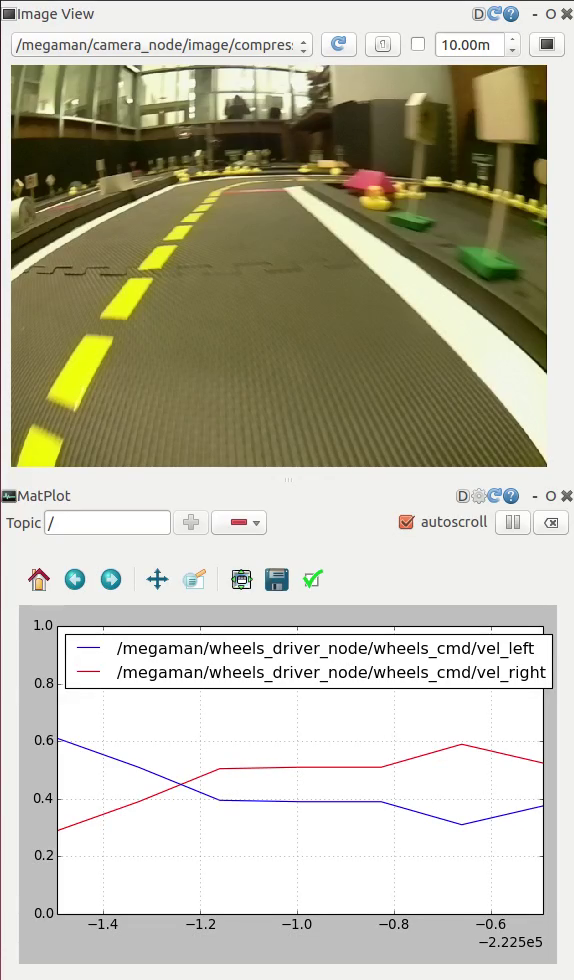
\includegraphics[width=\textwidth,height=0.8\textheight,keepaspectratio]{videos/lane_control_IO.png}}{videos/lane_control_IO.mp4}
		\end{column}
	\end{columns}
\end{frame}

\begin{frame}{Computation Graph: Lane Following}
\todo{Decentralized implementation}
\todo{Modularity}
\begin{center}
\includedot[width=\textwidth,height=0.8\textheight,keepaspectratio]{dot/lane_following}%
\end{center}
\end{frame}

\begin{frame}{Line Detection Node}
\framesubtitle{Hang Zhao}
	\begin{columns}
		\begin{column}{0.6\textwidth}
			\todo{Graph and zoom in. Add picture.}
		\end{column}
		\begin{column}{0.4\textwidth}
		  \movie[showcontrols=false]{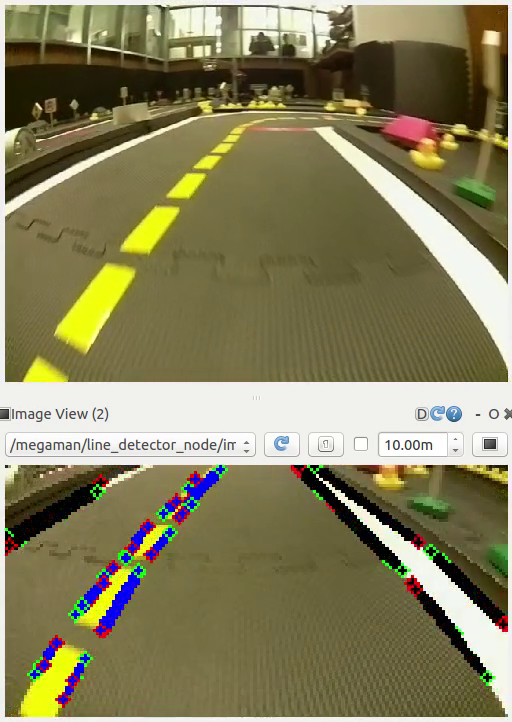
\includegraphics[width=\textwidth,height=0.8\textheight,keepaspectratio]{videos/line_detection.png}}{videos/line_detection.mp4}
		\end{column}
	\end{columns}
\end{frame}

\begin{frame}{Ground Projection Node}
\framesubtitle{Dr. Changhyun Choi}
	\begin{columns}
		\begin{column}{0.6\textwidth}
			\todo{Graph and zoom in. Add picture.}
		\end{column}
		\begin{column}{0.4\textwidth}
		  \movie[showcontrols=false]{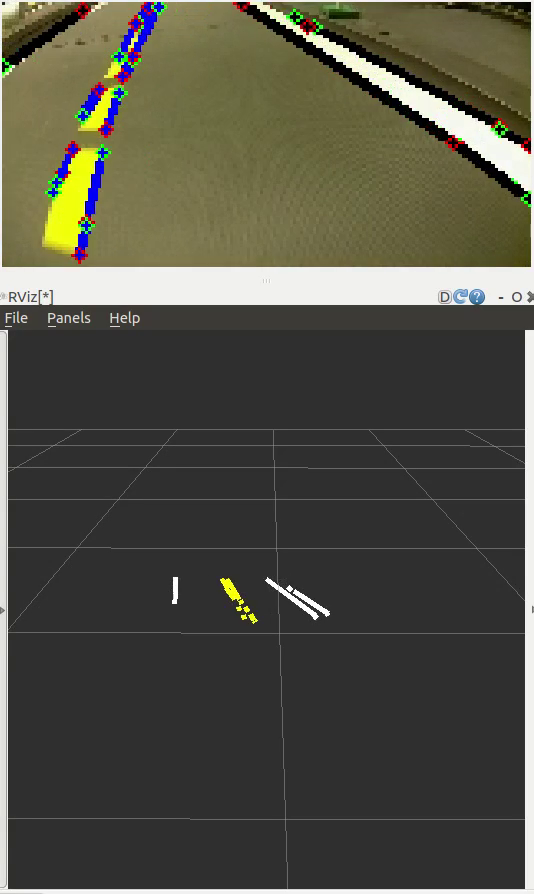
\includegraphics[width=\textwidth,height=0.8\textheight,keepaspectratio]{videos/ground_projection.png}}{videos/ground_projection.mp4}
		\end{column}
	\end{columns}
\end{frame}

\begin{frame}{Lane Filter Node}
\framesubtitle{Dr. Liam Paull}
	\begin{columns}
		\begin{column}{0.6\textwidth}
			\todo{Graph and zoom in. Add picture.}
		\end{column}
		\begin{column}{0.4\textwidth}
		  \movie[showcontrols=false]{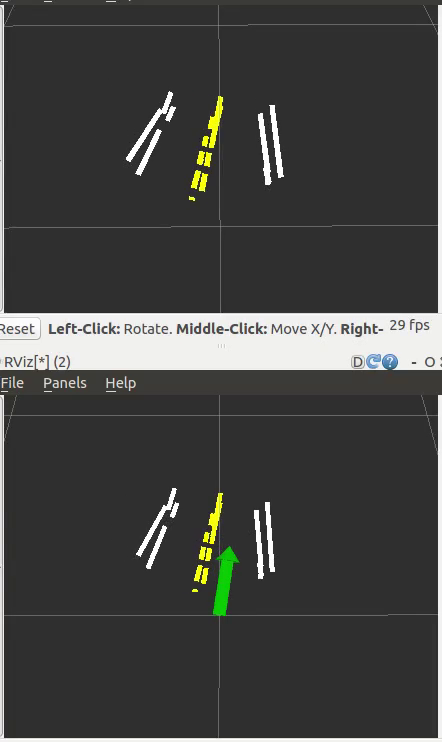
\includegraphics[width=\textwidth,height=0.8\textheight,keepaspectratio]{videos/lane_filter.png}}{videos/lane_filter.mp4}
		\end{column}
	\end{columns}
\end{frame}

\begin{frame}{Lane Control Node}
\framesubtitle{Steven Chen}
	\begin{columns}
		\begin{column}{0.6\textwidth}
			\todo{Graph and zoom in. Add picture.}
		\end{column}
		\begin{column}{0.4\textwidth}
		  \movie[showcontrols=false]{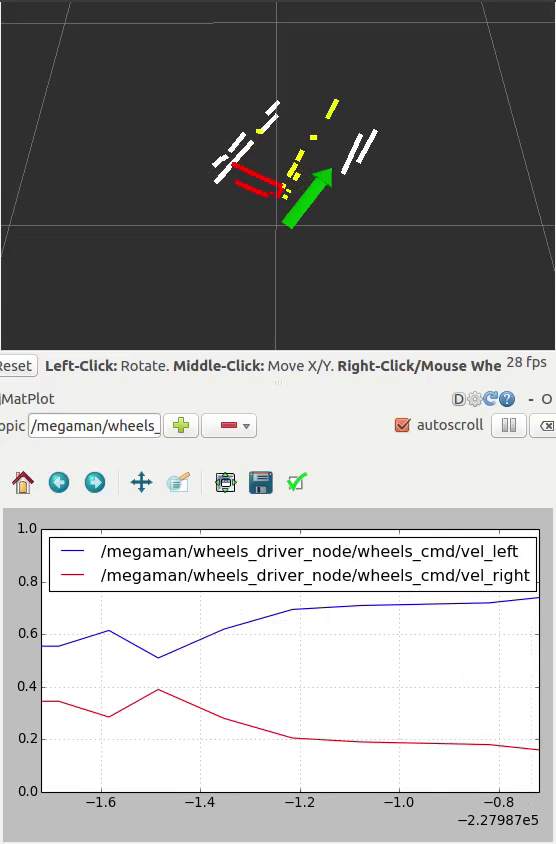
\includegraphics[width=\textwidth,height=0.8\textheight,keepaspectratio]{videos/lane_control.png}}{videos/lane_control.mp4}
		\end{column}
	\end{columns}
\end{frame}

\begin{frame}{Putting Them Together}
	\begin{center}
	  \movie[showcontrols=false]{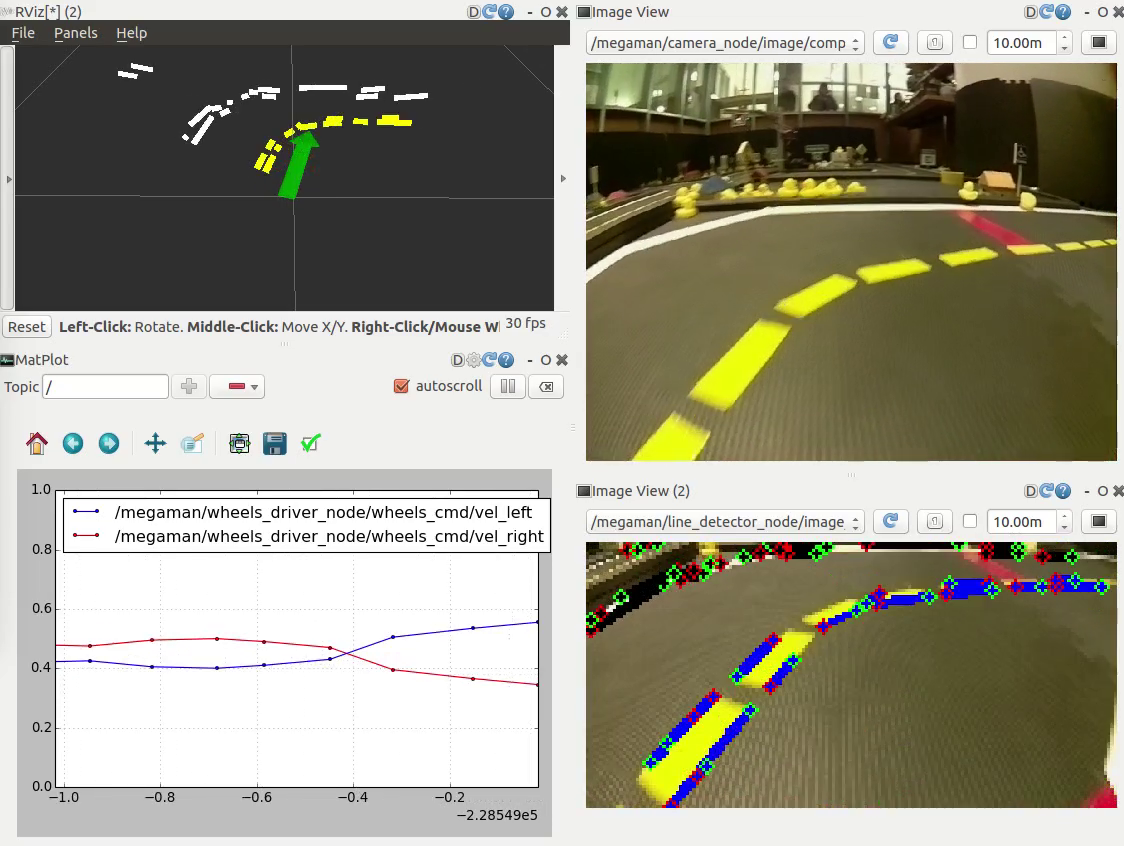
\includegraphics[width=\textwidth,height=0.8\textheight,keepaspectratio]{videos/lane_following_all.png}}{videos/lane_following_all.mp4}
	\end{center}
\end{frame}

\begin{frame}{Duckietown Architecture}
\begin{center}
	\includedot[width=\textwidth,height=0.8\textheight,keepaspectratio]{dot/Duckietown_ROS_Diagram}%
  \todo{Add mini summary of why we need middleware/ROS. How it helped.}
\end{center}

\end{frame}

\section{ROS Concept Overview}
\begin{frame}[label=overview]{Overview}
%	\tableofcontents
	\tableofcontents[sectionstyle=show/shaded,subsectionstyle=show/shaded/shaded]
\end{frame}


\begin{frame}{Nodes and Topics}
	\begin{columns}[c]
		\begin{column}{0.5\textwidth}
			%\todo[inline]{Graph. What is a node? Node/Edge explaination.}
			%\todo[inline]{Topic example with images. command plots etc.}
			\begin{itemize}
				\item Nodes:
					\begin{itemize}
					\item Executables (\texttt{python} or \texttt{C++})
					\item Each node is a process
					\item Publishes/Subscribes to Topics
					\end{itemize}
				\item Topics:
					\begin{itemize}
					\item Passes information between nodes
					\item Topic type defined by messages
					\item Support many-to-many communication
					\end{itemize}
			\end{itemize}
		\end{column}
		\begin{column}{0.5\textwidth}
			% \centering
			\includedot[width=\textwidth,height=0.8\textheight,keepaspectratio]{dot/node_and_topic}
%			\todo[inline]{Add two way communication figure}
%			\todo[inline]{Oval and Square are inversed on the diagram.... Fix this.}
		\end{column}
	\end{columns}
\end{frame}

\begin{frame}{ROS Master}
	\begin{columns}[T]
		\begin{column}{0.6\textwidth}
%			\todo[inline]{Transparnet on which machine running which code.}
			\begin{itemize}
			\item Handles communication between nodes
			\item Connects publisher and subscriber
			\item Traffic does \alert{not} go through the master once connected
			\item TCP/IP connection
			\item Command:
				\begin{itemize}
					\item Start a master: \inline{roscore}
				\end{itemize}
			\end{itemize}
		\end{column}
		\begin{column}{0.4\textwidth}
			\centering
			\includegraphics[width=\textwidth]{fig/tele_operator.jpg}
		\end{column}
	\end{columns}
  \todo{Consider more specific examples?}
  \todo{Specify machines}
	\only<1>{\includedot[width=\textwidth,height=\textheight,keepaspectratio]{dot/master_1}}
	\only<2>{\includedot[width=\textwidth,height=\textheight,keepaspectratio]{dot/master_2}}
	\only<3>{\includedot[width=\textwidth,height=\textheight,keepaspectratio]{dot/master_3}}
	\only<4>{\includedot[width=\textwidth,height=\textheight,keepaspectratio]{dot/master_4}}
	\only<5>{\includedot[width=\textwidth,height=\textheight,keepaspectratio]{dot/master_5}}
\end{frame}

\begin{frame}{Commandline Tools and Demo (Joystick)}
	\begin{columns}
		\begin{column}{0.5\textwidth}
      \todo{Add roscore here}
			\begin{itemize}
				\item Start a node:\\\inline{rosrun pkg_name node_exec}
				\item List all nodes:\\\inline{rosnode list}
				\item Info of a node:\\\inline{rosnode info node_name}
				\item List all topics:\\\inline{rostopic list}
				\item Info of a topic:\\\inline{rostopic info topic_name}
				\item Listen to a topic:\\\inline{rostopic echo topic_name}
				\item View communication graph:\\\inline{rqt_graph}
			\end{itemize}
		\end{column}
		\begin{column}{0.5\textwidth}
			\centering
			Live demo here.
			\todo[inline]{Terminals are scary}
			\todo[inline]{Package are not introduced.}
			\todo[inline]{Use camera and rqt graph as an example}
			\todo[inline]{rostopic hz}
		\end{column}
	\end{columns}
\end{frame}

\begin{frame}{Messages}
	\begin{columns}
		\begin{column}{0.7\textwidth}
			\begin{itemize}
				\item Message defines the type of a topic
				\item Syntax for \texttt{.msg} files:\\%
					Single value field: \inline{field_type field_name}\\%
					Fixed-length field: \inline{field_type[n] field_name}\\%
					Variable-length field: \inline{field_type[] field_name}
				\item Primitive Type: \inline{bool}, \inline{string}, \inline{float32}, \inline{int32}, \inline{time}, ... etc
				\item Common message packages:
					\begin{itemize}
						\item \inline{std_msgs}: 
						\item \inline{geometry_msgs}:
						\item \inline{sensor_msgs}:
					\end{itemize}
			\end{itemize}
      \todo{Too busy}
		\end{column}
		\begin{column}{0.3\textwidth}
			\centering
			%\includegraphics[width=\textwidth]{}
		\end{column}
	\end{columns}
\end{frame}

\begin{frame}{Parameters}
  \todo{Add intro to parameter server}
	\begin{columns}
		\begin{column}{1.0\textwidth}
			\begin{itemize}
				\item Kept on the parameter server (initialized with master)
				\item Persist until the master is killed
				\item Can be set/get at run time
					\begin{itemize}
						\item Commandline:\\\inline{rosparam set param_name}\\\inline{rosparam get param_name}
						\item Python:\\\pyinline{rospy.set_param(param_name,param_value)}\\\pyinline{rospy.get_param(param_name,default_value)}
					\end{itemize}
				\item Can be load/dump to yaml files:\\\inline{rosparam load file_name [namespace]}\\\inline{rosparam dump file_name [namespace]}
				\item Great namespace support with \inline{~}
			\end{itemize}
			\todo[inline]{Introduce yaml file. Maybe show an example.}
			\todo[inline]{Do we need intro to linux terminal?}
		\end{column}
		% \begin{column}{0.4\textwidth}
		% 	TODO: yaml file example
		% \end{column}
	\end{columns}
\end{frame}

\begin{frame}{Commandline Tools and Demo for Parameters}
	\begin{columns}
		\begin{column}{0.5\textwidth}
			\begin{itemize}
				\item List parameters:\\\inline{rosparam list}
				\item Get parameter:\\\inline{rosparam get param_name}
				\item Set parameter:\\\inline{rosparam set param_name}
				\item Dump parameters into file:\\\inline{rosparam dump file_name [namespace]}
				\item Read parameters from file:\\\inline{rosparam load file_name [namespace]}
			\end{itemize}
		\end{column}
		\begin{column}{0.5\textwidth}
			\centering
      Demo
		\end{column}
	\end{columns}
\end{frame}

%\begin{frame}{Services}
%	TODO
%\end{frame}

\begin{frame}{Launch File}
	\begin{columns}
		\begin{column}{0.6\textwidth}
			\begin{itemize}
				\item XML format file that can:
					\begin{itemize}
						\item Launch nodes and set their names
						\item Set/Load parameters
						\item Remap topics
						\item Include other launch files
						\item Take and pass arguments from commandline
					\end{itemize}
				\item Tags:
					\begin{itemize}
						\item \inline{<launch>}
						\item \inline{<group>}
						\item \inline{<arg>}
						\item \inline{<node>}
						\item \inline{<param>},\inline{<rosparam>}
						% \item \inline{<machine>}
						\item \inline{<include>}
					\end{itemize}
				% \item In Duckietown:
				% 	\begin{itemize}
				% 		\item Each node has one elemental launch file
				% 		\item Documents the I/O of a node
				% 		\item Standard interfaces through \inline{<arg>}
				% 	\end{itemize}
			\end{itemize}
		\end{column}
	\begin{column}{0.4\textwidth}
		\centering
		TODO: example using camera.launch and joystick.launch
		DEMO: command line argument --args --ros-arg --find etc
		%\includegraphics[width=\textwidth]{}
		\end{column}
	\end{columns}
\end{frame}

\begin{frame}{Attribute and Elements \texttt{<node>}}
	\begin{columns}
		\begin{column}{0.6\textwidth}
			\begin{itemize}
				\item Key attributes:
					\begin{itemize}
						\item \inline{pkg} 
						\item \inline{type} 
						\item \inline{name} 
						\item \inline{args} 
						\item \inline{machine} 
						\item \inline{ns} 
						\item \inline{output} 
					\end{itemize}
				\item Key elements:
					\begin{itemize}
						\item \inline{<remap>}
						\item \inline{<rosparam>}
						\item \inline{<param>}
					\end{itemize}
			\end{itemize}
		\end{column}
		\begin{column}{0.4\textwidth}
			\centering
			%\includegraphics[width=\textwidth]{}
		\end{column}
	\end{columns}
\end{frame}

%\begin{frame}{Launch File Elements}
%	\begin{columns}
%		\begin{column}{0.6\textwidth}
%			\begin{itemize}
%				\item 
%			\end{itemize}
%		\end{column}
%		\begin{column}{0.4\textwidth}
%			\centering
%			%\includegraphics[width=\textwidth]{}
%		\end{column}
%	\end{columns}
%\end{frame}

\begin{frame}{Joystick (Remote Control)}
	\begin{columns}
		\begin{column}{0.4\textwidth}
			\begin{itemize}
				\item \inline{joy}
				\item \inline{joy_mapper_node}
				\item \inline{wheels_trimmer_node}
				\item \inline{wheels_driver_node}
			\end{itemize}
		\end{column}
		\begin{column}{0.6\textwidth}
			\centering \includedot[width=\textwidth,height=\textheight,keepaspectratio]{dot/joystick}
		\end{column}
	\end{columns}
\end{frame}

\begin{frame}{Packages}
\begin{columns}
	\begin{column}{0.6\textwidth}
		\begin{itemize}
			\item Packages are organization tools for:
			\begin{itemize}
				\item Functionality
				\item Build and runtime dependencies
				\item Namespaces
			\end{itemize}
			\item Key Files (TODO: More details on these three key files?)
				\begin{itemize}
					\item CMakeLists.txt
					\item package.xml
					\item setup.py
				\end{itemize}
			\item Tools
				\begin{itemize}
					\item \mintinline{bash}{roscd}
					\item \mintinline{bash}{rospack profile}
					\item \mintinline{bash}{rospack depends}
					\item TODO: examples
				\end{itemize}
		\end{itemize}
	\end{column}
	\begin{column}{0.4\textwidth}
		\centering
		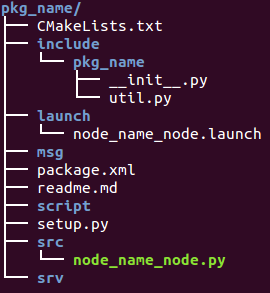
\includegraphics[width=\textwidth]{fig/pkg_tree.png}
	\end{column}
\end{columns}
\end{frame}

\section{Code Examples}
\begin{frame}[label=overview]{Overview}
%	\tableofcontents
	\tableofcontents[sectionstyle=show/shaded,subsectionstyle=show/shaded/shaded]
\end{frame}
% \begin{frame}{Camera (Data Processing)}
% 	\begin{columns}
% 		\begin{column}{0.42\textwidth}
% 			\begin{itemize}
% 				\item \inline{camera_node}
% 				\item \inline{decoder_node}
% 				\item \inline{cam_info_reader_node}
% 				\item \inline{intrinsic_calibration_file}
% 			\end{itemize}
% 		\end{column}
% 		\begin{column}{0.58\textwidth}
% 			\centering
% 			\includedot[width=\textwidth,height=\textheight,keepaspectratio]{dot/camera}
% 		\end{column}
% 	\end{columns}
% \end{frame}


% \begin{frame}{Publisher Node Code Example}
% 	\framesubtitle{\texttt{publisher\_node.py}}
% 	\inputminted{python}{snippet/publisher_node.py}
% 	\begin{itemize}
% 		\item Initialize a node: \pyinline{rospy.init_node(node_name)}
% 		\item Create publisher: \pyinline{rospy.Publisher(topic_name,msg_type,queue_size)}
% 	\end{itemize}
% 	\todo[inline]{Explain queue\_size}
% 	\todo[inline]{Should use rostopic list, rosnode list before writing own node.}
% 	\todo[inline]{Should just use the timer version. Better form, less messy. rospy.spin() not necessary}
% \end{frame}

\begin{frame}{Publisher Node Code Example with Timer}
	\framesubtitle{\texttt{publisher\_node\_timer.py}}
	\inputminted{python}{snippet/publisher_node_timer.py}
	\begin{itemize}
	\item Timer is more elegant than a while loop
	\item Start a timer: \pyinline{rospy.Timer(duration,callback)}
	\end{itemize}
\end{frame}

\begin{frame}{Subscriber Node Code Example}
	\framesubtitle{\texttt{subscriber\_node.py}}
	\inputminted{python}{snippet/subscriber_node.py}
	\begin{itemize}
		\item Create a subscriber: \pyinline{rospy.Subscriber(topic_name,callback)}
	\end{itemize}
\end{frame}

\begin{frame}{Parameter Code Example}
	\framesubtitle{\texttt{publisher\_node\_param.py}}
	\inputminted{python}{snippet/publisher_node_param.py}
	% \begin{itemize}
	% 	\item Read parameter from parameter server:\\\pyinline{rospy.get_param(param_name,default_value)}
	% \end{itemize}
\end{frame}

\begin{frame}{Message Definition Examples}
	\begin{itemize}
		\item \texttt{Duckie.msg} defines the name, state, and pose of a duckie.
		\inputminted{python}{snippet/Duckie.msg}
		\item \texttt{DuckieList.msg} contains a list of duckies.
		\inputminted{python}{snippet/DuckieList.msg}
		\item Look up msg definition:\\\inline{rosmsg show pkg_name/msg_name}
	\end{itemize}
	\todo[inline]{Double check consistency}
\end{frame}

\begin{frame}{Message Usage in Publisher Code Example}
	\framesubtitle{publisher\_node\_msg.py}
	\inputminted{python}{snippet/publisher_node_msg.py}
	\todo[inline]{Use student name}
\end{frame}

\begin{frame}{Message Usage in Subscriber Code Example}
	\framesubtitle{subscriber\_node\_msg.py}
	\inputminted{python}{snippet/subscriber_node_msg.py}
\end{frame}


\begin{frame}{Resources}
  \begin{columns}
	\begin{column}{0.6\textwidth}
	  \begin{itemize}
		\item TODO: links to ROS tutorial and wiki
	  \end{itemize}
	\end{column}
  \begin{column}{0.4\textwidth}
		\centering
		%\includegraphics[width=\textwidth]{}
		% \digraph[scale=0.5]{abc}{a->b->c;}
	\end{column}
  \end{columns}
\end{frame}

% \begin{frame}{Duckietown ROS Diagram}
%	\digraph[scale=0.2]{aaa}{\input{dot/duckietown}}
	% \includedot[scale=0.8]{dot/test}
% \end{frame}

%\begin{frame}{Snippet}
%	\begin{itemize}[<+->]
%		\item Hey
%		\inputminted{python}{snippet/test.py}
%		\item Ho \mintinline{python}{import numpy as np}
%	\end{itemize}
%\end{frame}

\end{document}